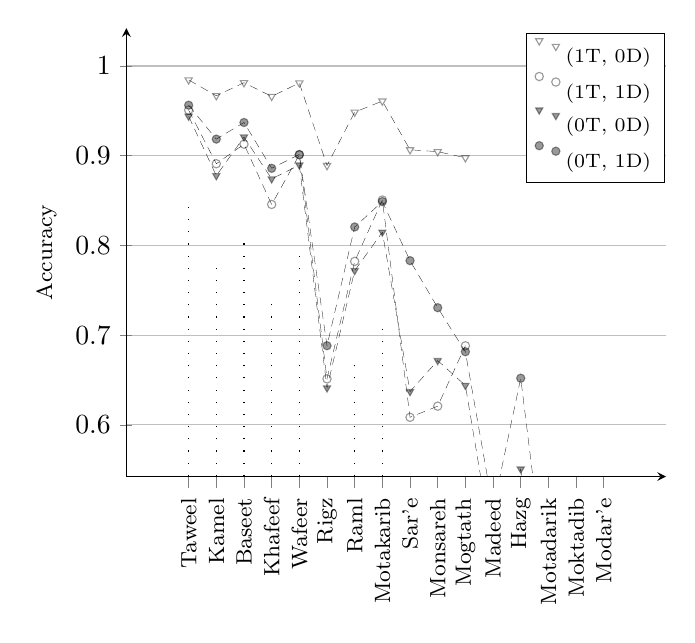
\begin{tikzpicture}[scale=1]
  \begin{axis}[
    axis x line = bottom,
    axis y line = left,
    ymajorgrids = true,
    ybar,
    enlargelimits=0.15,
    legend style={at={(0.87,0.99)},
      anchor=north,legend columns=1},
    ylabel={Accuracy},
    ylabel style = {font=\footnotesize},
    symbolic x coords={Taweel, Kamel, Baseet, Khafeef, Wafeer, Rigz, Raml, Motakarib, Sar'e, Monsareh, Mogtath, Madeed, Hazg, Motadarik, Moktadib, Modar'e},
    xtick=data,
    xticklabel style = {font=\footnotesize},
    nodes near coords align={vertical},
    x tick label style={rotate=90, anchor=east},
    bar width=2pt,
    ymin=0.6,
    ]

    % trimmed no-diacritic (Empty Triangle)
    \addplot[mark=triangle, every mark/.append style={rotate=180},
    thin, only marks, mark size=1.5pt, point meta=explicit symbolic, opacity=0.4]
    coordinates {
      % (1T, 0D)
      (Wafeer,    0.9811213222198475)       
      (Monsareh,  0.9045746962115797)       
      (Mogtath,   0.897708216880939 )       
      (Motakarib, 0.9609120521172638)       
      (Kamel,     0.966898378020523 )       
      (Taweel,    0.9844991757498216)       
      (Sar'e,     0.9066397034041119)       
      (Raml,      0.9485771342985522)       
      (Rigz,      0.8889925373134329)       
      (Khafeef,   0.9661488673139158)       
      (Baseet,    0.9814341393906374) 
      (Madeed,     0)  
      (Hazg,       0) (Motadarik,  0) 
      (Moktadib,   0) 
      (Modar'e,    0)
    };

    % trimmed diacritic (Empty Circle)
    % (1T, 1D)
    \addplot[mark=o, thin, only marks, mark size=1.5pt, point
    meta=explicit symbolic, opacity=0.4]
    coordinates{
      (Wafeer,     0.9009759920210871)
      (Monsareh,   0.6208005718370264)
      (Mogtath,    0.6880939072107323)
      (Motakarib,  0.8506281991624011)
      (Kamel,      0.8910956636875207)
      (Taweel,     0.9508402430922914)
      (Sar'e,      0.6083586113919784)
      (Raml,       0.7822016974538193)
      (Rigz,       0.6512042062415196)
      (Khafeef,    0.8456957928802589)
      (Baseet,     0.9128703742508696)
    };


    % full no-diacritic (Full Triangle)
    % (0T, 0D)
    \addplot[mark=triangle*, every mark/.append style={rotate=180},
    thin, only marks, mark size=1.5pt, point meta=explicit symbolic, opacity=0.4]
    coordinates {
      (Wafeer,    0.889584964761159)
      (Monsareh,  0.6716101694915254)
      (Madeed,    0.45979899497487436)
      (Mogtath,   0.6439135381114903)
      (Motakarib, 0.8148088917319687)
      (Kamel,     0.8776972469479428)
      (Taweel,    0.9439529481540059)
      (Sar'e,     0.6370179948586119)
      (Raml,      0.7719209325899645)
      (Rigz,      0.64107517849643)
      (Khafeef,   0.8741908607319105)
      (Baseet,    0.9208657001620072)
      (Moktadib,  0.16326530612244897)
      (Hazg,      0.5506493506493506)
      (Modar'e,   0.0)
      (Motadarik, 0.28)
    };

    % full diacritic (Full Circle)
    % (0T, 1D)
    \addplot[mark=*, thin, only marks, mark size=1.5pt, point
    meta=explicit symbolic, opacity=0.4]
    coordinates {
      (Wafeer,    0.9014024346835623)
      (Monsareh,  0.7305790960451978)
      (Madeed,    0.5062814070351759)
      (Mogtath,   0.6814562002275313)
      (Motakarib, 0.8488725411802335)
      (Kamel,     0.9185383195083638)
      (Taweel,    0.9563337122522612)
      (Sar'e,     0.7830334190231363)
      (Raml,      0.8205778003041054)
      (Rigz,      0.6881982360352793)
      (Khafeef,   0.8859834647183235)
      (Baseet,    0.9370664229634861)
      (Moktadib,  0.3673469387755102)
      (Hazg,      0.6519480519480519)
      (Modar'e,   0.08333333333333333)
      (Motadarik, 0.40190476190476193)
    };

    \legend{
      {\scriptsize (1T, 0D)},
      {\scriptsize (1T, 1D)},
      {\scriptsize (0T, 0D)},
      {\scriptsize (0T, 1D)},
    }

    % Dotted line
    \draw[loosely dotted] (axis cs:Wafeer,    0) -- (axis cs:Wafeer,     0.789584964761159);
    \draw[loosely dotted] (axis cs:Monsareh,  0) -- (axis cs:Monsareh,   0.5208005718370264);
    \draw[loosely dotted] (axis cs:Mogtath,   0) -- (axis cs:Mogtath,    0);
    \draw[loosely dotted] (axis cs:Motakarib, 0) -- (axis cs:Motakarib,  0.7148088917319687);
    \draw[loosely dotted] (axis cs:Kamel,     0) -- (axis cs:Kamel,      0.7776972469479428);
    \draw[loosely dotted] (axis cs:Taweel,    0) -- (axis cs:Taweel,     0.8439529481540059);
    \draw[loosely dotted] (axis cs:Sar'e,     0) -- (axis cs:Sar'e,      0.5083586113919784);
    \draw[loosely dotted] (axis cs:Raml,      0) -- (axis cs:Raml,       0.6719209325899645);
    \draw[loosely dotted] (axis cs:Rigz,      0) -- (axis cs:Rigz,       0.54107517849643);
    \draw[loosely dotted] (axis cs:Khafeef,   0) -- (axis cs:Khafeef,    0.7456957928802589);
    \draw[loosely dotted] (axis cs:Baseet,    0) -- (axis cs:Baseet,     0.8128703742508696);
    \draw[loosely dotted] (axis cs:Moktadib,  0) -- (axis cs:Moktadib,   0);
    \draw[loosely dotted] (axis cs:Madeed,    0) -- (axis cs:Madeed,     0.35979899497487436);
    \draw[loosely dotted] (axis cs:Hazg,      0) -- (axis cs:Hazg,       0.4506493506493506);
    \draw[loosely dotted] (axis cs:Modar'e,   0) -- (axis cs:Modar'e,    0);
    \draw[loosely dotted] (axis cs:Motadarik, 0) -- (axis cs:Motadarik,  0.18);


    % connecting  models accuracies

    % Empty Triangle
    % (1T, 0D)
    \draw[line width=0.1pt, densely dashed]
    (axis cs:Taweel,        0.9844991757498216)
    -- (axis cs:Kamel,      0.966898378020523 )
    -- (axis cs:Baseet,     0.9814341393906374)
    -- (axis cs:Khafeef,    0.9661488673139158)
    -- (axis cs:Wafeer,     0.9811213222198475)
    -- (axis cs:Rigz,       0.8889925373134329)
    -- (axis cs:Raml,       0.9485771342985522)
    -- (axis cs:Motakarib,  0.9609120521172638)
    -- (axis cs:Sar'e,      0.9066397034041119)
    -- (axis cs:Monsareh,   0.9045746962115797)
    -- (axis cs:Mogtath,    0.897708216880939 );

   % Empty Circle
   % (1T, 1D)
   \draw[line width=0.1pt, densely dashed]
   (axis cs:Taweel,        0.9508402430922914)
   -- (axis cs:Kamel,      0.8910956636875207)
   -- (axis cs:Baseet,     0.9128703742508696)
   -- (axis cs:Khafeef,    0.8456957928802589)
   -- (axis cs:Wafeer,     0.9009759920210871)
   -- (axis cs:Rigz,       0.6512042062415196)
   -- (axis cs:Raml,       0.7822016974538193)
   -- (axis cs:Motakarib,  0.8506281991624011)
   -- (axis cs:Sar'e,      0.6083586113919784)
   -- (axis cs:Monsareh,   0.6208005718370264)
   -- (axis cs:Mogtath,    0.6880939072107323);


    % Full Triangle
    % (0T, 0D)
    \draw[line width=0.1pt, densely dashed]
    (axis cs:Taweel,        0.9439529481540059)
    -- (axis cs:Kamel,      0.8776972469479428)
    -- (axis cs:Baseet,     0.9208657001620072)
    -- (axis cs:Khafeef,    0.8741908607319105)
    -- (axis cs:Wafeer,     0.889584964761159)
    -- (axis cs:Rigz,       0.64107517849643)
    -- (axis cs:Raml,       0.7719209325899645)
    -- (axis cs:Motakarib,  0.8148088917319687)
    -- (axis cs:Sar'e,      0.6370179948586119)
    -- (axis cs:Monsareh,   0.6716101694915254)
    -- (axis cs:Mogtath,    0.6439135381114903)
    -- (axis cs:Madeed,     0.4597989949748743)
    -- (axis cs:Hazg,       0.5506493506493506)
    -- (axis cs:Motadarik,  0.28)
    -- (axis cs:Moktadib,   0.1632653061224489)
    -- (axis cs:Modar'e,    0.0               );


   % Full Circle
   % (0T, 1D)
   \draw[line width=0.1pt, densely dashed]
   (axis cs:Taweel,        0.9563337122522612)
   -- (axis cs:Kamel,      0.9185383195083638)
   -- (axis cs:Baseet,     0.9370664229634861)
   -- (axis cs:Khafeef,    0.8859834647183235)
   -- (axis cs:Wafeer,     0.9014024346835623)
   -- (axis cs:Rigz,       0.6881982360352793)
   -- (axis cs:Raml,       0.8205778003041054)
   -- (axis cs:Motakarib,  0.8488725411802335)
   -- (axis cs:Sar'e,      0.7830334190231363)
   -- (axis cs:Monsareh,   0.7305790960451978)
   -- (axis cs:Mogtath,    0.6814562002275313)
   -- (axis cs:Madeed,     0.5062814070351759)
   -- (axis cs:Hazg,       0.6519480519480519)
   -- (axis cs:Motadarik,  0.4019047619047619)
   -- (axis cs:Moktadib,   0.3673469387755102)
   -- (axis cs:Modar'e,    0.0833333333333333);

  \end{axis}
\end{tikzpicture}
